\documentclass[pdftex,12pt,a4paper]{article}

\usepackage{graphicx}  
\usepackage[margin=2.5cm]{geometry}
\usepackage{breakcites}
\usepackage{indentfirst}
\usepackage{pgfgantt}
\usepackage{pdflscape}
\usepackage{float}
\usepackage{epsfig}
\usepackage{epstopdf}
\usepackage[cmex10]{amsmath}
\usepackage{stfloats}
\usepackage{multirow}
\usepackage{karnaugh-map}
\usepackage{amssymb}
\usepackage{amsbsy}
\usepackage{placeins}
\usepackage[utf8]{inputenc}
\usepackage[english]{babel}


\renewcommand{\refname}{REFERENCES}
\linespread{1.3}

\usepackage{mathtools}
%\newcommand{\HRule}{\rule{\linewidth}{0.5mm}}
\thispagestyle{empty}
\begin{document}
\begin{titlepage}
\begin{center}
\textbf{}\\
\textbf{\Large{ISTANBUL TECHNICAL UNIVERSITY}}\\
\vspace{0.5cm}
\textbf{\Large{COMPUTER ENGINEERING DEPARTMENT}}\\
\vspace{2cm}
\textbf{\Large{BLG 222E\\ COMPUTER ORGANIZATION\\ FINAL PROJECT REPORT}}\\
\vspace{2.8cm}
\begin{table}[ht]
\centering
\Large{
\begin{tabular}{lcl}
\textbf{PROJECT NO}  & : & 4 \\
\textbf{PROJECT DATE}  & : & 14.07.2020 \\
\textbf{GROUP NO}  & : & 36 \\
\end{tabular}}
\end{table}
\vspace{1cm}
\textbf{\Large{GROUP MEMBERS:}}\\
\begin{table}[ht]
\centering
\Large{
\begin{tabular}{rcl}
150170087  & : & Sırrı Batuhan ÇOKSAK(Group Representative) \\
150170069  & : & Furkan Yusuf GÜRAY \\
150170039  & : & Fatih MURAT \\
150160142  & : & Ekin Zuhat YAŞAR \\
\end{tabular}}
\end{table}
\vspace{2.8cm}
\textbf{\Large{SPRING 2020}}

\end{center}

\end{titlepage}

\thispagestyle{empty}
\addtocontents{toc}{\contentsline {section}{\numberline {}FRONT COVER}{}}
\addtocontents{toc}{\contentsline {section}{\numberline {}CONTENTS}{}}

\setcounter{tocdepth}{4}
\tableofcontents
\clearpage


\section{INTRODUCTION}
\par

In the final project, we were expected to design and implement software-based (microprogrammed) control unit for the architecture in the Figure-1.

\begin{figure}[h]
    	\centering
    	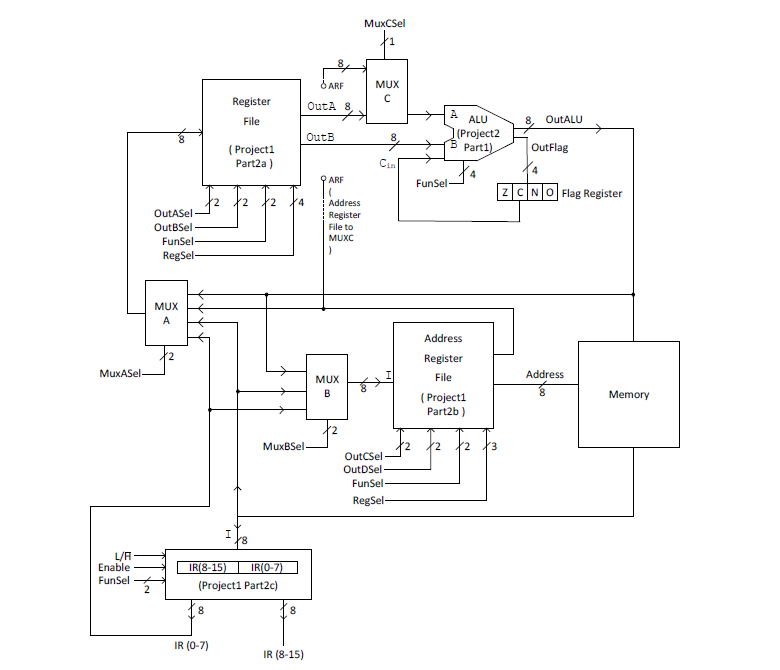
\includegraphics[width=0.9\textwidth]{template.png}	
    	\caption{Template architecture}
    	\label{temp arch}
\end{figure}

\setcounter{page}{1}

\section{DESIGN}
In the project we were given 19 different opcodes in the Figure2, we analyzed the opcodes and decided our mapping format which would be "1 + opcode + 00" which means that we will be using 4 line of micro-instructions to perform the operation of the opcode, the added 1 bit to the start of the mapping will aid some issues which will be discussed in discussion part of the report. 

\begin{figure}[H]
    	\centering
    	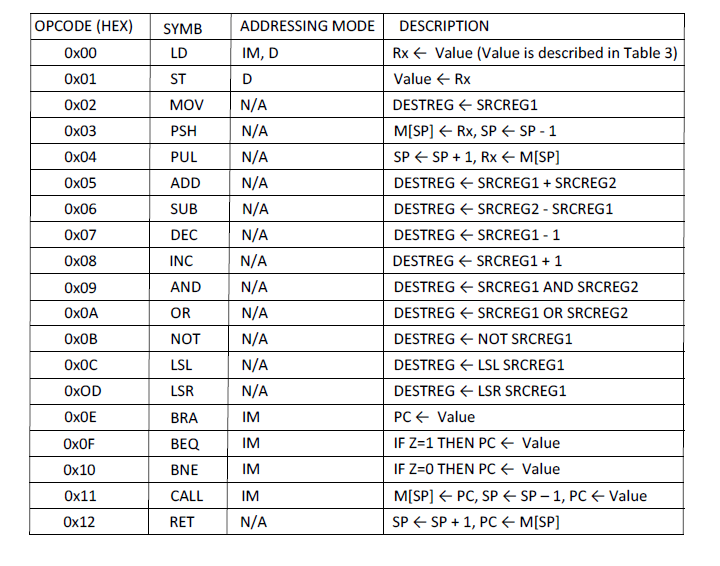
\includegraphics[width=0.9\textwidth]{table1.png}	
    	\caption{Operation Codes}
    	\label{opcodes table}
\end{figure}

Furthermore, in order to perform that 19 different operations we required 24 different micro-instructions.
Tables at the end of the file Table 1 and 2 shows the  micro-operations and their objective; table 3,4,5 shows the Symbolic micro-program of our design. 

In addition we designed our ROM to have 24 bit data in each address and 8 bit address values, we separated those 24 bit data as follows:
first 4 bit  for F1,
second 4 bit for F2,
third 4 bit for F3,
fourth 4 bit for CD+BR,
and the last 8 bit for address values. During our design we did not require the F3 operation field however if in the future the design requires additional micro-operations the field  can be easily used since its completely empty. Furthermore designing the field bits are address values and CD+BR field in 4 bit or 8 bit
gives us a clean ROM values since the every 4 bit is represented as hex values in ROM first bit in the ROM means  F1 field in hexadecimal form, this form can be easily debugged and read since it is not needed to convert whole value to binary from in order to read specific field from the value.  In addition, when designing CD and BR we used the lessons slide as a base however since the design of the cpu is different we 
omitted the unnecessary pieces and left them as blank so if in the future they are needed, they can be implemented.

\clearpage

\section{RESULT}
As a result of the project, we verified our implementation using the test code which is given in the project pdf file and with our own tests. There was not any contradiction between the expected and obtained results. Test code that we have tried over our implementation in the project pdf file is shown in the Figure 3.

\begin{figure}[H]
    	\centering
    	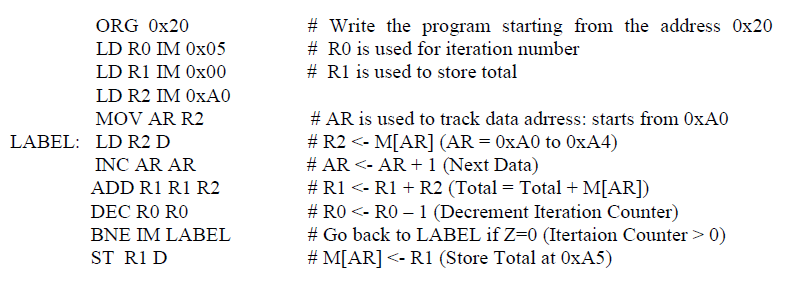
\includegraphics[width=0.9\textwidth]{test.png}	
    	\caption{Test code from the project file}
    	\label{test code}
\end{figure}

Our design is shown as in the Figure-4.

\begin{figure}[H]
    	\centering
    	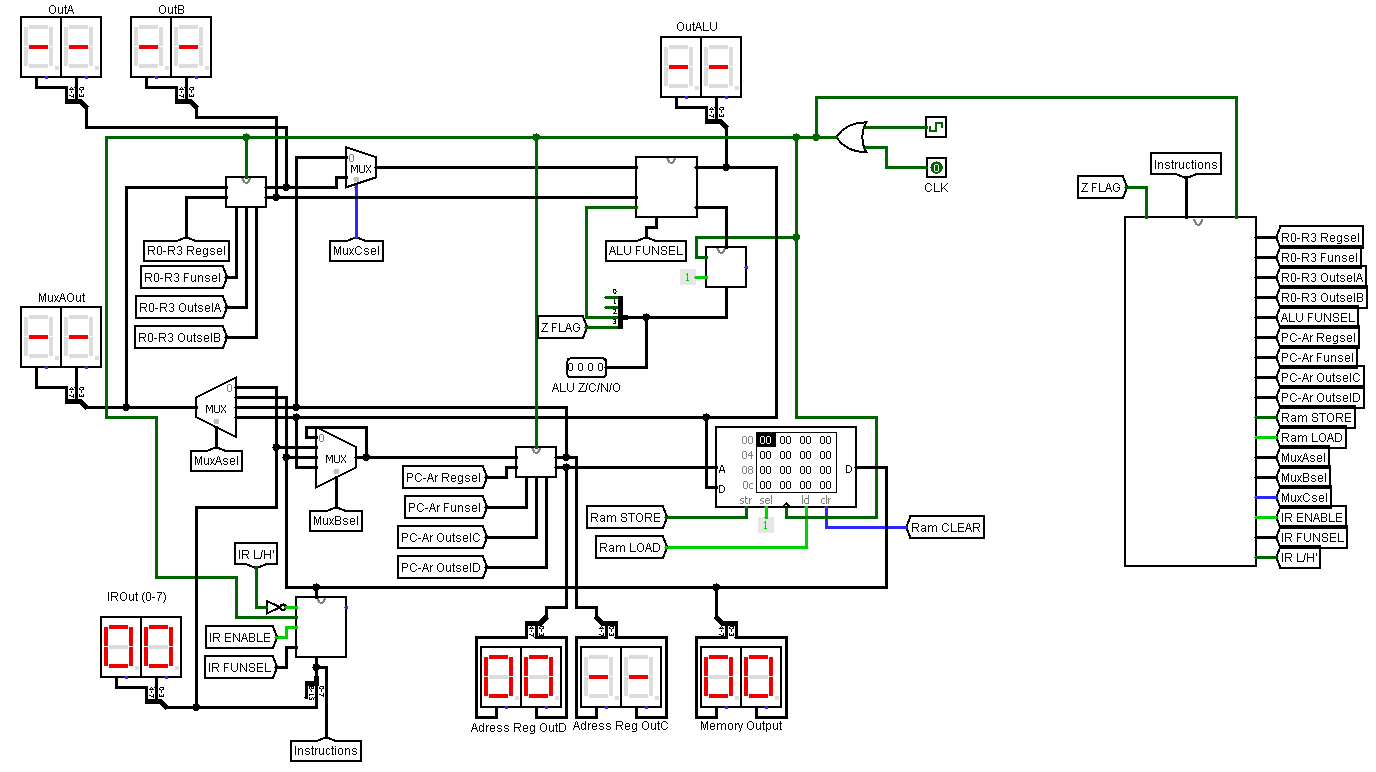
\includegraphics[width=0.9\textwidth]{final.png}	
    	\caption{Final Implementation of Our Design}
    	\label{implement}
\end{figure}

\newpage

\section{DISCUSSION}

In this final project, we were expected to implement a software-control unit using our project 1\&2 implementations and a few design ideas from project 3. We had micro-instructions and operations to deal with.Tackling new problems that rose with micro-operation based design was challenging at first. We have a few assumptions, for example register call for PC having 2 different codes was problematic for us. At first we tried using an OR gate to accommodate two codes representing PC but that proved to be wrong, OR gate would give an error when it had two X's as inputs. In addition when mapping our opcode we used the following format "1 opcode 00", as mentioned in the Design part last 2 bits represent how many address we will have when performing that operation which is 4, adding 1 to the first bit in the address allows us the keep the fetch micro-operation at the address 00000000 which means that when the project file is opened control address  register will show the address 00000000 which means that the CPU will do the fetch operation next. Also if somehow CAR shows an unused address from ROM the hexa value of 000000 will be performed which means NO operation unconditional jump to 00000000 which is the fetch line meaning that the system will recover in case of an error as such


\section{CONCLUSION}

In conclusion this project helped define the idea of a software-control unit in our minds. Specifically how different it is to a hardwired counterpart. We had to use a completely different approach to our OPCODE design both in taking and executing the micro instructions. Instead of a time slot based on clock we used micro-operations from our ROM, which meant we were able to do similar tasks with way less wiring and gates, effectively cutting down total part cost. 
\clearpage
\section{APPENDIX}
\begin{table}[h]
    \centering
    \begin{tabular}{|c|c c c|}
    \hline
    F1 & Microoperation  & Symbol & Description \\ \hline
    0000 &    NONE		   &       NONE    &         	NONE      \\
    0001 &    Reg$<$-Reg 	 &     MOV	 &           MOVE    \\
    0010 &    Rx$<$-IR(0-7)	 &     LD	     &       LOAD    \\
    0011 &    PC$<$-IR(0-7)   &    LPC	 &           LOAD to PC        \\
    0100 &    AR$<$-IR(0-7)  &     LAR	     &       LOAD  to AR        \\
    0101 &    Reg$<$-M(AR)     &   RD	   &         READ,  Load from memory	        \\
    0110 &    M(AR)$<$-Rx	   &   STR	    &        Store, write  to memory	        \\
    0111 &    M(SP)$<$-PC	   &   CLL	    &        CALL       \\
    1000 &    PC$<$-M(SP)	   &   RTR	       &     RETURN            \\
    1001 &    M(SP)$<$-Reg	&      PSH	  &          PUSH	            \\
    1010 &    Reg $<$-M(SP)	   &   PLL	         &   PULL	       \\
    1011 &    AReg$<$-AReg+1    &  SIN       &       	(Self increment) INCREMENT DESTREG            \\
    1100 &    AReg$<$- AReg-1   &  SDC	  &          (Self  decrement) DECREMENT DESTREG        \\
    1101 &    SP$<$-SP-1	   &   DSP	 &           DECREMENT SP            \\
    1110 &    SP$<$-SP+1	   &   ISP	 &           INCREMENT SP       \\ \hline
    \end{tabular}
    \caption{Microoperation table of $F_1$}
    \label{mp f1}
\end{table}

\begin{table}[H]
    \centering
    \begin{tabular}{|c|c c c|}
    \hline
    F2 & Microoperation  & Symbol & Description \\ \hline
    0000 &    NON			   &       NON    &         	NONE                 \\
    0001 &    Reg$<$-Reg+Reg	 &         ADD	        &     ADD               \\
    0010 &    Reg$<$-Reg-Reg	 &         SUB	     &       SUB         \\
    0011 &    Reg$<$-Reg \& Reg    &      AND	 &             AND               \\
    0100 &    Reg$<$-Reg $|$ Reg  &        OR	     &       OR                         \\
    0101 &    REG$<$- NOT REG    &       NOT	   &         NOT	        \\
    0110 &    REG $<$- LSL REG	   &   LSL	    &        LOGİCAL LEFT SHİFT	        \\
    0111 &    REG$<$-  LSR REG	   &   LSR	    &        LOGİCAL right shift        \\
    1000 &    IR(8-15)$<$-M(PC)	   &   FUP	       &     FETCH UP         \\
    1001 &    IR(7-0)$<$-M(PC)	&      FDW	  &          FETCH DOWN          \\
    1010 &    PC$<$-PC+1		   &       IPC	 &           INCREMENT PC	             \\ \hline
    \end{tabular}
    \caption{Microoperation table of $F_2$}
    \label{mp f2}
\end{table}

\begin{table}[h]
    \centering
    \begin{tabular}{|c|c|c|c|c|c|c|}
    \hline
    ROM address	&Microop&	F1&	F2&	F3&	CD-BR&		Address field \\\hline
00000000 &	FETCH UP&	0000 &	1000 &		0000    &	0000	 &		00000001 \\ \hline	
00000001 &	INC PC	&	0000 &	1010 &		0000	&   0000	 &		00000010 \\ \hline
00000010 &	FETCHDOWN&	0000 & 	1001 &		0000	&   0000	 &		00000011 \\ \hline
00000011 &	INC PC	&	0000 &	1010 &		0000	&   0011	 &		XXXXXXXX \\ \hline
10000000 &	NON	    & 0000 &	0000 &		0000	&   0100	 &		10000010 \\ \hline
10000001 &	LOAD	&	0010 &	0000 &		0000	&   0000	 &		00000000 \\ \hline
10000010 &	READ	&	0101 &	0000 &		0000	&   0000	 &		00000000 \\ \hline
10000011 &	UNUSED  &&&&& \\ \hline
10000100 &	NON	    &	0000&	0000    &	0000	&   0100	 &		10000110 \\ \hline
10000101 &	NON	    &	0000&	0000    &	0000	&   0000	 &		00000000\\ \hline
10000110 &	STORE	&	0110&	0000    &	0000	&   0000	 &		00000000\\ \hline
10000111 &	UNUSED  &&&&&                                   \\ \hline
10001000 &	MOVE	&	0001  &	0000    &	0000 &		0000	 &		00000000\\ \hline
10001001 &	UNUSED  &&&&&                                       \\ \hline
10001010 &	UNUSED  &&&&&                                        \\ \hline
10001011 &	UNUSED  &&&&&                                 			\\ \hline
10001100 &	DEC SP  &	1101    &	0000    &	0000 &		0000	 &		10001101\\ \hline
10001101 &	PUSH    &	1001    &	0000    &	0000 &		0000	 &		00000000\\ \hline
10001110 &	UNUSED&&&&&\\ \hline
10001111 &	UNUSED&&&&&\\ \hline
10010000 &	PULL    &	1010 &		0000 &		0000 &		0000	 &		10010001\\ \hline
10010001 &	INC  SP &	1110 &		0000 &		0000 &		0000	 &		00000000\\ \hline
10010010 &	UNUSED  &&&&&\\ \hline
10010011 &	UNUSED  &&&&&\\ \hline
10010100 &	ADD	    &	0000 &		0001 &		0000 &		0000	 &		00000000\\ \hline
10010101 &	UNUSED  &&&&&\\ \hline
10010110 &	UNUSED  &&&&&\\ \hline
10010111 &	UNUSED  &&&&&\\ \hline
10011000 &	SUB	    &	0000 &		0010 &		0000 &		0000	 &		00000000\\ \hline
10011001 &	UNUSED  &&&&&\\ \hline
10011010 &	UNUSED  &&&&&\\ \hline
10011011 &	UNUSED  &&&&&\\ \hline
    \end{tabular}
    \caption{Symbolic Microprogram-1}
    \label{mp1}
\end{table}

\begin{table}[h]
    \centering
    \begin{tabular}{|c|c|c|c|c|c|c|}
    \hline
    ROM address	&Microop&	F1&	F2&	F3&	CD-BR&		Address field \\\hline
10011100 &	MOV	    &	0001 &		0000 &		0000 &		0000	 &		10011101\\ \hline
10011101 &	SELF DEC&	1100 &		0000 &		0000 &		0000	 &		00000000		 \\\hline
10011110 &	UNUSED  &&&&&\\ \hline
10011111 &	UNUSED  &&&&&\\ \hline
10100000 &	MOV	    &		0001 &		0000 &		0000 &		0000	 &		10100001\\ \hline
10100001 &	SIN		&	  1011 &		0000 &		0000 &		0000	 &		00000000\\ \hline
10100010 &	UNUSED  &&&&&\\\hline
10100011 &	UNUSED  &&&&&\\\hline
10100100 &	AND     &	 0000 &		0011 &		0000 &		0000	 &		00000000\\ \hline
10100101 &	UNUSED  &&&&&\\\hline
10100110 &	UNUSED  &&&&&\\\hline
10100111 &	UNUSED  &&&&&\\\hline
10101000 &	OR      &		0000 &		0100 &		0000 &		0000	 &		00000000\\ \hline
10101001 &	UNUSED  &&&&&\\\hline
10101010 &	UNUSED  &&&&&\\\hline
10101011 &	UNUSED  &&&&&\\\hline
10101100 &	NOT     &		0000 &		0101 &		0000 &		0000	 &		00000000\\\hline
10101101 &	UNUSED  &&&&&\\\hline
10101110 &	UNUSED  &&&&&\\\hline
10101111 &	UNUSED  &&&&&\\\hline
10110000 &	LSL     &		0000 &		0110 &		0000 &		0000	 &		00000000\\\hline
10110001 &	UNUSED  &&&&&\\\hline
10110010 &	UNUSED  &&&&&\\\hline
10110011 &	UNUSED  &&&&&\\\hline
10110100 &	LSR     &		0000 &		0111 &		0000 &		0000	 &		00000000\\\hline
10110101 &	UNUSED  &&&&&\\\hline
10110110 &	UNUSED  &&&&&\\\hline
10110111 &	UNUSED  &&&&&\\\hline
10111000 &	NON     &		0000 &		0000 &		0000 &		0100	 &		00000000\\\hline
10111001 &	LPC     &	   0011 &		0000 &		0000 &		0000	 &		00000000\\\hline
10111010 &	UNUSED  &&&&&\\\hline
10111011 &	UNUSED  &&&&&\\\hline
   \end{tabular}
    \caption{Symbolic Microprogram-2}
    \label{mp2}
\end{table}




\begin{table}[h]
    \centering
    \begin{tabular}{|c|c|c|c|c|c|c|}
    \hline
    ROM address	&Microop&	F1&	F2&	F3&	CD-BR&		Address field \\\hline
10111100 &	NON     &  0000 &		0000 &		0000 &		0100	 &		00000000 \\\hline
10111101 &	NON     &  0000 &		0000 &		0000 &		1100	 &		10111111\\\hline
10111110 &	NON     &  0000 &		0000 &		0000 &		0000	 &		00000000\\\hline
10111111 &	LPC     &  0011 &		0000 &		0000 &		0000	 &		00000000\\\hline
11000000 &	NON     &  0000 &		0000 &		0000 &		0100	 &		00000000 \\\hline
11000001 &	NON     &  0000 &		0000 &		0000 &		1100	 &		00000000\\\hline
11000010 &	LPC     &  0011 &		0000 &		0000 &		0000	 &		00000000\\\hline
11000011 &	UNUSED  &&&&&\\\hline
11000100 &	NON     &  0000 &		0000 &		0000 &		0100	 &		00000000\\\hline
11000101 &	DEC SP	&	1101 &		0000 &		0000 &		0000	 &		11000110\\\hline
11000110 &	CALL	&	0111 &		0000 &		0000 &		0000	 &		11000111\\\hline
11000111 &	LPC		&  0011 &		0000 &		0000 &		0000	 &		00000000\\\hline
11001000 &	RETURN	&  1000 &		0000 &		0000 &		0000	 &		11001001\\\hline
11001001 &	INC SP	&	1110 &		0000 &		0000 &		0000	 &		00000000\\\hline
11001011 &	UNUSED  &&&&&\\\hline
11001100 &	UNUSED  &&&&&\\\hline


   \end{tabular}
    \caption{Symbolic Microprogram-3}
    \label{mp3}
\end{table}



\end{document}









 
